\section{Implementation}

This section will describe the design and engineering processes that were used while implementing our system, based on the requirements described above. In order to simplify and structure its description, the system will first be broken down into its different logical components.


\subsection{High-Level System Architecture}
The various requirements and corresponding program functionality of our system can be broken down into four main areas: the 7-segment display, the keypad, the ADC and the PWM timer. Despite the overall system having significant complexity, there is a very limited number of states for the overall system, with the transition between them being very well defined. A state diagram showing the three states, along with the name of their transitions can be seen in Figure 1.


% Messing around with hand-made FSM diagrams.
\begin{tikzpicture}[shorten >=1pt,node distance=4cm,on grid,auto] 
   \node[state,initial] (sleep)  {$Sleep$}; 
   \node[state] (input_target)	[below right=of sleep]	{$Input$}; 
   \node[state] (match_voltage) 	[below left=of sleep]	{$Match $};
   \path[->]
   	(sleep)
   		edge node {$WakeUp()$} (input_target);
   \path[->] ([yshift=1ex]input_target.west) (input_target) edge node {$Sleep()$} (sleep);
	\path 
	(input_target) 
		edge node {$StartMatching()$} (match_voltage)
   		%edge node [swap loop right] {$Reset()$} ()
   	(match_voltage)
   		edge node {$Reset()$} (input_target)
   		edge node {$Sleep()$} (sleep);  


\end{tikzpicture}


\begin{center}
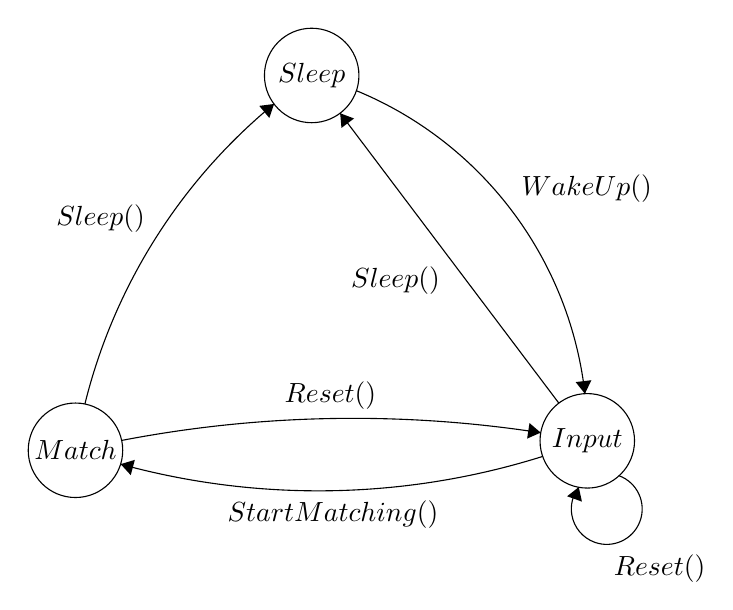
\begin{tikzpicture}[scale=0.2]
\tikzstyle{every node}+=[inner sep=0pt]
\draw [black] (27.3,-15.7) circle (3);
\draw (27.3,-15.7) node {$Sleep$};
\draw [black] (44.8,-38.9) circle (3);
\draw (44.8,-38.9) node {$Input$};
\draw [black] (12.3,-39.5) circle (3);
\draw (12.3,-39.5) node {$Match$};
\draw [black] (30.138,-16.666) arc (67.58113:6.47412:23.704);
\fill [black] (44.65,-35.91) -- (45.06,-35.05) -- (44.06,-35.17);
\draw (40.6,-22.9) node [right] {$WakeUp()$};
\draw [black] (41.969,-39.89) arc (-72.54178:-105.34292:47.471);
\fill [black] (15.17,-40.38) -- (15.81,-41.08) -- (16.07,-40.11);
\draw (28.65,-42.69) node [below] {$StartMatching()$};
\draw [black] (15.234,-38.875) arc (100.91105:81.20424:77.764);
\fill [black] (41.84,-38.38) -- (41.13,-37.77) -- (40.98,-38.76);
\draw (28.49,-36.92) node [above] {$Reset()$};
\draw [black] (42.99,-36.5) -- (29.11,-18.1);
\fill [black] (29.11,-18.1) -- (29.19,-19.03) -- (29.99,-18.43);
\draw (35.47,-28.7) node [left] {$Sleep()$};
\draw [black] (46.808,-41.113) arc (69.9454:-218.0546:2.25);
\draw (49.39,-46.08) node [below] {$Reset()$};
\fill [black] (44.26,-41.84) -- (43.52,-42.42) -- (44.46,-42.76);
\draw [black] (12.898,-36.561) arc (166.10108:129.45639:35.822);
\fill [black] (24.91,-17.51) -- (23.97,-17.63) -- (24.61,-18.4);
\draw (16.74,-24.77) node [left] {$Sleep()$};
\end{tikzpicture}
\end{center}


\begin{tikzpicture}[shorten >=1pt,node distance=2cm,on grid,auto] 
   \node[state,initial] (q_0)   {$q_0$}; 
   \node[state] (q_1) [above right=of q_0] {$q_1$}; 
   \node[state] (q_2) [below right=of q_0] {$q_2$}; 
   \node[state,accepting](q_3) [below right=of q_1] {$q_3$};
    \path[->] 
    (q_0) edge  node {0} (q_1)
          edge  node [swap] {1} (q_2)
    (q_1) edge  node  {1} (q_3)
          edge [loop above] node {0} ()
    (q_2) edge  node [swap] {0} (q_3) 
          edge [loop below] node {1} ();
\end{tikzpicture}
